\documentclass{standalone}
\usepackage{tikz}
\usepackage{ctex,siunitx,ninecolors}
\setCJKmainfont{Noto Serif CJK SC}
\usepackage{tkz-euclide}
\usepackage{amsmath}
\usetikzlibrary{patterns, calc}
\usetikzlibrary {decorations.pathmorphing, decorations.pathreplacing, decorations.shapes,}
\begin{document}
\small
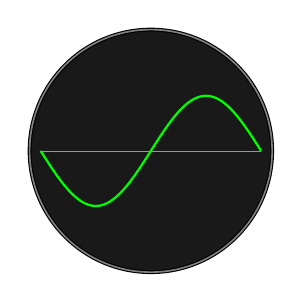
\begin{tikzpicture}[>=latex,scale=0.7]
  \draw[double=gray,fill=black!90] (2,0) circle (2.2);
  \draw[thick,green](0,0) sin (1,-1) cos (2,0) sin (3,1) cos (4,0);
  \draw[very thin,green](0,0)--(4,0);
\end{tikzpicture}
\end{document}